\chapter{Caso de Uso} \label{ch:cdu}

O presente capítulo visa explicar o caso de uso da ontologia. O caso de uso da
ontologia é uma simulação de uma parte da vida dos personagens. Eles
encontram-se observando um jogo de futebol e cada um torce para um time.
Entretanto, antes desse caso de uso ser abordado na seção~\ref{ch:cdu:svc}
será falado como a ontologia foi testada juntamente com a plataforma \jason.
A seção~\ref{ch:cdu:tbc} explica as ferramentas desenvolvidas para testar a base
de crenças e, consequentemente, a ontologia. Elas são duas uma interativa e
outra não interativa que serve como uma especie de teste unitário.

\section{Teste da Base de Crenças} \label{ch:cdu:tbc}

Os testes da base de crenças tem como finalidade checar se a utilização normal
esta acontecendo da maneira esperada. Assim, eles fazem testes de inserção,
recuperação, remoção e listagem. A listagem é feita implementando a interface
\emph{Iterable} da plataforma Java e é usada, principalmente, quando a
interface gráfica da plataforma \jason esta em modo depuração e
exibindo a base de crenças.

\begin{figure}
	\begin{center}
		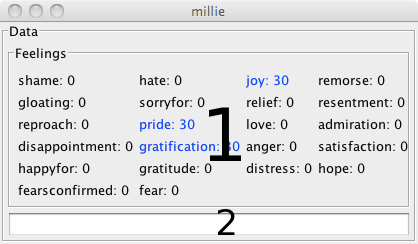
\includegraphics[width=70mm]{figuras/introductionDF.png}
	\end{center}
	\caption{Interface para mostrar os sentimentos dos agentes.}
	\label{fig:introducaoDF}
\end{figure}

A primeira aplicação de teste desenvolvida foi de maneira interativa conforme
pode ser observado na Figura~\ref{fig:introducaoDF}. A aplicação permite que o
usuário escreva as crenças do agente em um campo texto (área 2 na figura) e
esse é enviado diretamente para a base de crença do agente. A área 1 na mesma
figura é utilizada para demostrar a valência das emoções.
Essas informações podem aparecer em: preto, se não houve alteração com o ciclo
anterior; azul, se houve um aumento; vermelho, se houve uma diminuição do
valor.

\begin{figure}
	\begin{center}
		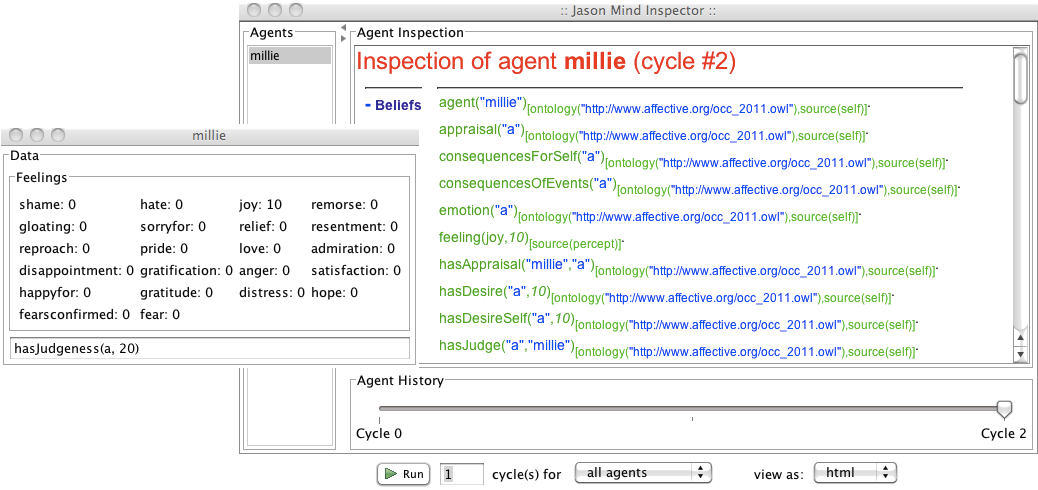
\includegraphics[width=150mm]{figuras/beforeLastInsertionOfPride.png}
		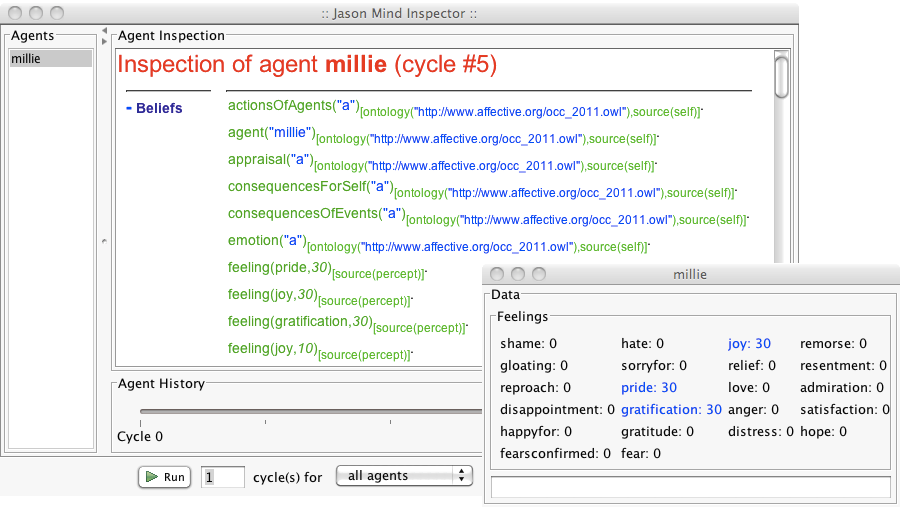
\includegraphics[width=150mm]{figuras/afterLastInsertionOfPride.png}
	\end{center}
	\caption{Exemplo de utilização criando uma emoção de orgulho.}
	\label{fig:testeJasonIntBase}
\end{figure}

Na Figura~\ref{fig:testeJasonIntBase} estão representados dois momentos da
criação de uma emoção de orgulho da parte do usuário. Na parte de cima, o
agente tem configurado uma avaliação de e sobre si próprio. Além disso, a
avaliação tem probabilidade nula ou irrelevante e o desejo para si mesmo foi
considerado com o valor 10. Esse valor poderia ser qualquer número inteiro,
mas se fosse negativo ao invés de alegria (\emph{joy}) o resultado atual seria
sofrimento (\emph{distress}). No campo de texto, o usuário irá inserir a
última relação para ser construída a percepção de orgulho.

Na parte de baixo da Figura~\ref{fig:testeJasonIntBase} pode se ver o
resultado obtido para a inserção da última crença. Conforme pode ser visto,
foi necessário três ciclos deliberativos para o agente ter a percepção do
sentimento. Na verdade, essa percepção não veio de um novo ciclo de simulação
rodando e sim que o agente acrescentou uma nova crença dizendo que havia um
passo novo então foi feita a avaliação das emoções quanto a necessidade de
se criar a percepção afetiva. Se fosse um passo normal da simulação, não se
teria na base de crenças duas percepções \emph{feeling} sobre uma emoção
porque a todo novo passo as percepções são limpas.

Na Listagem~\ref{lst:testeJasonIntBase} pode ser observado uma configuração
para se rodar a presente aplicação\footnote{Veja a seção
\ref{sec-jason-overview} na página~\pageref{sec-jason-overview}
para ver uma introdução sobre esse tipo de arquivo.}. O ambiente na linha 4
espera que todos os agentes (quantidade informada no parâmetro 3) mandem
uma ação para prosseguir. O simulador espera pelo tempo (em milissegundos)
configurado no primeiro parâmetro por essas ações, caso não venha ignora o
agente e segue para o próximo ciclo. O segundo parâmetro permite que seja
configura um número que representa o último passo de simulação e no quarto
parâmetro permite configurar se uma segunda ação enviada no mesmo passo de
simulação é para ser enfileirada ou resultar em erro (essa é a opção atual).

\begin{center}
    \begin{minipage}{130mm}
	\lstset{linewidth=130mm}
	\lstinputlisting[frame=trbl, caption=Arquivo de projeto do \jason para a
aplicação interativa de teste, label=lst:testeJasonIntBase]{../../sampletConsole/eoaus.mas2j}
    \end{minipage}
\end{center}

A agente millie configurada da linha 7 à 11 utiliza opções do \jason para
alterar a base de crença sendo utilizada (\emph{beliefBaseClass}),
arquitetura do agente (\emph{agentArchClass}) e o próprio agente
(\emph{agentClass}). Dessas alterações, a mudança da base de crença e da
classe do agente foram explicadas na seção~\ref{ch:p:ipjo}. Assim, para o
presente exemplo a mudança da arquitetura na linha 9 foi realizada para criar
e atualizar a janela que exibe os dados emotivos.

Cabe chamar a atenção que na linha 8 da Listagem~\ref{lst:testeJasonIntBase}
foi usada a ontologia afetiva desenvolvida somente. Assim, para o agente
utilizar as emoções ainda é necessário incluir as configurações do valor
excedido para se ter a emoção presente via código do agente. Uma amostra do
código utilizado para se fazer isso pode ser vista na
Listagem~\ref{lst:testeJasonIntSetup} e todo o código pode ser encontrado no
repositório no \emph{GitHub}\footnote{http://github.com/rlucca/Maro}.

\lstset{linewidth=80mm}
\begin{wrapfigure}{l}{90mm}
	\begin{lstlisting}[frame=trbl,
caption=Parte do código do agente para aplicação interativa de teste,
label=lst:testeJasonIntSetup]
step(0)[source(percept),source(self)].

agent(millie).

hasSetup(millie, setup1).
hasThreshold(setup1, 0).
hasThresholdType(setup1, "Joy").

hasSetup(millie, setup2).
hasThreshold(setup2, 0).
hasThresholdType(setup2, "Distress").
	\end{lstlisting}
\end{wrapfigure}

A Listagem~\ref{lst:testeJasonIntSetup} mostra crenças que o agente terá
no inicio da simulação na plataforma \jason. Essas são populadas na memória
de acordo com a classe especificada na linha 8 da
Listagem~\ref{lst:testeJasonIntBase}. Esse processo já foi explicado na
seção~\ref{ch:p:ipjo}, a crença de \emph{step} como não
consta na ontologia será carregada na base de crenças padrão do \jason e as
demais mostradas serão inseridas na ontologia. Como pode ser observado, esse
processo é bastante transparente para o usuário.

Note também que o usuário precisou definir o limite para uma emoção virar
sentimento. No exemplo esse valor esta sendo definido como zero para que a
potência e a valência sejam iguais. Se for definido algum outro valor, a
potência será o valor total da emoção e esse valor não é de conhecimento do
agente. Ele conhece apenas a valência que será a diferença do valor total
menos o limite para ativação definido pela relação \emph{hasThreshold}. Por
exemplo, se o limite da pena (\emph{sorryFor}) é 6 e o valor atual é 8 então o
agente terá o sentimento com o valor 2 que será expresso por uma crença da
seguinte forma ``feeling("sorryFor",2).''.

%%%% fim da explicacao da aplicação interativa %%%%%

\begin{center}
    \begin{minipage}{140mm}
	\lstset{linewidth=140mm}
	\lstinputlisting[frame=trbl, caption=Arquivo de projeto do \jason para a
aplicação não interativa de teste,
label=lst:testeJasonNIBase]{../../sampletSummary/eoaus.mas2j}
    \end{minipage}
\end{center}

A aplicação não interativa utiliza a Listagem~\ref{lst:testeJasonNIBase} para
configurar o seu projeto. O ambiente especificado na linha 4 possui os mesmos
parâmetros do anterior com o acréscimo de um novo que indica uma ontologia.
Essa ontologia serve para o ambiente conhecer as rotinas dos agentes na
simulação, como deve ser desenhado o mapa exibido e as posições iniciais dos
agentes. O agente millie aqui é o utilizado para os testes e os limiares de
ativação de emoção estão configurados para valores diferentes. Existe uma
variedade de testes para as propriedades de objeto ou de dados e para as
instâncias de classes, além de testes das conclusões esperadas na ontologia do
agente. Veja o código do agente no repositório disponível no
\emph{GitHub}\footnote{http://github.com/rlucca/Maro}.

\section{Assistindo um jogo de futebol} \label{ch:cdu:svc}

O caso de uso utilizado para demostrar a ontologia representa dois personagens
que se encontram no mesmo lugar e encontram-se assistindo ao mesmo jogo de
futebol. O jogo tem ao todo 60 turnos que representam os 90 minutos de um jogo
regulamentar. Em cada turno é sorteado um número randômico com probabilidade
de 1.67 de probabilidade para os times marcarem gol, isto é, há 98.33\% de
chance à cada turno de nada acontecer e o placar permanecer inalterado.

Esse exemplo aparentemente simples, propicia um cenário bastante rico para as
emoções por causa que um personagem pode ter diferentes emoções acontecendo.
Essas emoções são muitas vezes do ramo de consequências de eventos por esta
estar ligada com a desejabilidade do evento ou do ramo de ações de agentes que
tem haver com os padrões do agentes. Assim, os agentes que estão assistindo ao
jogo de futebol decidem no inicio da simulação os times que estarão torcendo e
ambos acreditam que seus times vão ganhar.

\begin{center}
    \begin{minipage}{140mm}
	\lstset{linewidth=140mm}
	\lstinputlisting[frame=trbl, caption=Arquivo de projeto do \jason para o
exemplo de futebol,
label=lst:soccer]{../../sampletSoccer/soccer.mas2j}
    \end{minipage}
\end{center}

A Listagem~\ref{lst:soccer} mostra o arquivo de projetos que cria dois agentes
um chamado ``watch1'' e ``watch2'', cada um com seu próprio código fonte.
Dessa forma, cada um desses agentes inclui em seus códigos as configurações
necessárias para utilizar o \emph{framework}. Um exemplo dessas configurações
é o limite de ativação para uma emoção virar sentimento. Outro exemplo é que
os times que participam do jogo são considerados pelos personagens como outros
agentes, dessa forma o time que eu torço pode ser considerado um ``agente
amigo'' e o time adversário um ``agente inimigo''.

Cabe salientar que cada um dos agentes realizam as mesmas avaliações sobre os
mesmos eventos. Esses eventos foram pensados como o estado atual do jogo
(Listagem~\ref{lst:soccerTeam}), o estado final do jogo
(Listagem~\ref{lst:soccerEnd1} e Listagem~\ref{lst:soccerEnd2}) e a marcação de um gol
(Listagem~\ref{lst:soccerGoal}). Esses são alguns exemplos escritos escritos
na plataforma \jason para exemplificar o \emph{framework} construído.

\begin{center}
    \begin{minipage}{120mm}
	\lstset{linewidth=120mm}
	\begin{lstlisting}[frame=trbl,
caption=Parte do código do agente referente à avaliação de gol,
label=lst:soccerGoal]
+?appraisalGoal
    :  goal(TEAM) & myPoints(TEAM, PF, _, _)
    <- ?fib(8-(PF+1), VAL);
       ?updateEmotion(prospectIrrelevant, "goal_myteam_pi", VAL);
       +removeEmotion("goal_myteam_pi").

+?appraisalGoal
    :  goal(TEAM) & myPoints(_, _, TEAM, PE)
    <- ?fib(PE+1, VAL);
       ?updateEmotion(prospectIrrelevant, "goal_enemyteam_pi", -VAL);
       +removeEmotion("goal_enemyteam_pi").

+?appraisalGoal
    : removeEmotion(INDIVIDIDUAL)
   <- ?removeEmotion(prospectIrrelevant, INDIVIDIDUAL);
      -removeEmotion(INDIVIDIDUAL).

+?appraisalGoal.
	\end{lstlisting}
    \end{minipage}
\end{center}

A Listagem~\ref{lst:soccerGoal} realiza o processamento das emoções sentidas
por um personagem quando um time marca um gol. Nessa primeira listagem, a 4
condições possíveis: gol do time que torço, gol do time adversário, gol já
não é mais percebido e não foi nenhum gol. As emoções envolvidas em gols foram
consideradas alegria e sofrimento. Assim, quando o agente percebe o mesmo pode
ficar alegre ou em agonia. As linhas 4 e 15 sera vista mais adiante por hora
basta saber que elas realizam a inserção, atualização ou remoção dos dados
guardados na ontologia.

A Listagem~\ref{lst:soccerTeam} é similar. Ela é responsável por inserir uma
emoção de esperança no agente com valoração 50 e inicia o calculo de
realização do evento assumindo o valor positivo 1. Após, a cada gol percebido
do próprio time esse valor é incrementado em 10 e se o gol for do time
adversário é feito o decremento. A emoção de esperança não sofre alteração
depois que é criada porque esta sendo considerado que as emoções são baseadas
na percepção dos eventos. Dessa forma, a esperança do jogo ser ganho só
termina quando há a percepção do encerramento do mesmo. O mesmo vale para a
emoção sentida em gols.

\begin{center}
    \begin{minipage}{130mm}
	\lstset{linewidth=130mm}
	\begin{lstlisting}[frame=trbl,
caption=Parte do código do agente referente ao andamento do jogo,
label=lst:soccerTeam]
+?appraisalTeam
    :  not(hasLikelihood("team_hope_prn", PROB)) & step(STEP) & STEP < 10
    <- ?updateEmotion(prospectNotRealized, "team_hope_prn", 50);
       +realizedCalculation(1).

+?appraisalTeam
    :  goal(TEAM) & myPoints(_,_, TEAM, _) // ponto que nao eh meu
    &  realizedCalculation(CALC)
    <- -realizedCalculation(CALC);
       +realizedCalculation(CALC-10).

+?appraisalTeam
    :  goal(TEAM) & myPoints(TEAM, _, _,_) // ponto que eh meu
    &  realizedCalculation(CALC)
    <- -realizedCalculation(CALC);
       +realizedCalculation(CALC+10).

+?appraisalTeam.
	\end{lstlisting}
    \end{minipage}
\end{center}

\begin{center}
    \begin{minipage}{140mm}
	\lstset{linewidth=140mm}
	\begin{lstlisting}[frame=trbl,
caption=Parte do código do agente referente à avaliação do final do jogo,
label=lst:soccerEnd1]
+?appraisalEndMatch
    :  realizedCalculation(CALC) & match(_,_)
    &  hasLikelihood("team_hope_prn", PROB)
    &  feeling(hope, HOPEVAL)
    <- ?removeEmotion(prospectNotRealized, "team_hope_prn");
       ?updateEmotion(prospectRealized, "team_satisfaction_pr", HOPEVAL, CALC);
       -realizedCalculation(CALC).

+?appraisalEndMatch
    :  realizedCalculation(CALC) & match(_,_)
    &  hasLikelihood("team_hope_prn", PROB)
    <- ?removeEmotion(prospectNotRealized, "team_hope_prn");
       -realizedCalculation(CALC).

+?appraisalEndMatch.
	\end{lstlisting}
    \end{minipage}
\end{center}

Nas Listagens~\ref{lst:soccerEnd1}~e~\ref{lst:soccerEnd2} são realizadas
avaliações depois do termino do jogo. O jogo pode terminar empatado ou um dos
dois times ganhar. Entretanto, para a primeira listagem basta que o jogo tenha
terminado para uma atitude ser tomada. Essa atitude é remoção da emoção de
esperança e a criação de uma nova emoção baseado na realização do jogo e no
valor atual da esperança. Sendo assim, um personagem pode ficar satisfeito ou
desapontado.

Já, a Listagem~\ref{lst:soccerEnd2} permite um personagem sentir-se feliz
por um resultado ou ficar com pena de seu time. Quando o time do personagem
tiver ganho o jogo ele pode sentir-se feliz ou neutro e quando o time perde
ele pode sentir-se com pena ou neutro da mesma forma. Esse valor de
neutralidade é porque o modelo de emoções só diz que a felicidade por alguém
ou a pena só serão sentidas quando o merecimento e o desejo do outro forem
ambas positivas ou ambas negativas.

\begin{center}
    \begin{minipage}{140mm}
	\lstset{linewidth=140mm}
	\begin{lstlisting}[frame=trbl,
caption=Parte do código do agente referente à avaliação do final do jogo,
label=lst:soccerEnd2]
+?appraisalEndMatchHappy
     : match(win, TEAM) & myPoints(TEAM, _, _, _)
     & not(hasAppraisal(NAME, "team_happy_foo"))
    <- .random(N); DE=math.round(N*20)-10; DT=20;
       ?updateEmotion(fortunesOfOthers, "team_happy_foo", DE, DT).

+?appraisalEndMatchHappy
     : match(lose, TEAM) & myPoints(TEAM, _, _, _)
     & not(hasAppraisal(NAME, "team_happy_foo"))
    <- .random(N); DE=math.round(N*20)-10;
       DT=-20; // eh negativo para implificar na emocao de pena
       ?updateEmotion(fortunesOfOthers, "team_happy_foo", DE, DT).

+?appraisalEndMatchHappy
     : match(draw, _) & myPoints(TEAM, _, _, _)
     & not(hasAppraisal(NAME, "team_happy_foo"))
    <- .random(N); DE=math.round(N*20)-10; DT=10;
       ?updateEmotion(fortunesOfOthers, "team_happy_foo", DE, DT).

+?appraisalEndMatchHappy.
	\end{lstlisting}
    \end{minipage}
\end{center}

As consultas de ``removeEmotion'' recebem o tipo de emoção e o nome do
indivíduo que deve ser removido. Com base nessas informações, as relações
que foram outrora inseridas são removidos da base de conhecimento e,
consequentemente, da base de crenças. Um exemplo é amostrado na
Listagem~\ref{lst:removeSample} no qual são removidas às relações de
merecimento, de desejo por outros, de qual pessoa esta sendo avaliada e que
esta avaliando.

\begin{center}
    \begin{minipage}{130mm}
	\lstset{linewidth=130mm}
	\begin{lstlisting}[frame=trbl,
caption=Amostra de remoção de emoção do tipo destino de outros,
label=lst:removeSample]
+?removeEmotion(fortunesOfOthers, INDIVIDUAL)
     : hasDeserved(INDIVIDUAL, OLDDE) & hasDesireOther(INDIVIDUAL, OLDDO)
     & hasPerson(INDIVIDUAL, TEAM)
    <- ?myName(NAME);
       -hasPerson(INDIVIDUAL, TEAM);
       -hasDeserved(INDIVIDUAL, OLDDE);
       -hasDesireOther(INDIVIDUAL, OLDDO);
       -hasAppraisal(NAME, INDIVIDUAL).

+?removeEmotion(fortunesOfOthers, INDIVIDUAL).
	\end{lstlisting}
    \end{minipage}
\end{center}

As consultas de ``updateEmotion'' funcionam de maneiras similares. Elas
removem e acrescentam uma outra relação para repor a mesma relação com outro
valor. Dessa forma, para a construção do exemplo tanto as atualizações como as
remoções foram agrupadas por grupo de emoções por causa que essa é a forma que
o próprio modelo agrupa remoções com regras similares. A Listagem~\ref{lst:update}
mostra a regra para o tipo de emoções que tem haver com a consequência dos
destinos dos outros. Sendo assim, as relações de merecimento, de nível de
desejo dos outros e de quem esta avaliando e que pessoa. Todo o código pode
ser consultado no repositório disponível via
\emph{GitHub}\footnote{http://github.com/rlucca/Maro}.

\begin{center}
    \begin{minipage}{130mm}
	\lstset{linewidth=130mm}
	\begin{lstlisting}[frame=trbl,
caption=Amostra de código referente as atualizações de emoções do tipo destino de outros,
label=lst:update]
+?updateEmotion(fortunesOfOthers, INDIVIDUAL, DESERVED, DESIREOTHER)
     : team(TEAM) & not(hasPerson(INDIVIDUAL, TEAM))
    <- ?myName(NAME);
       +hasAppraisal(NAME, INDIVIDUAL);
       +hasPerson(INDIVIDUAL, TEAM);
       +hasDeserved(INDIVIDUAL, DESERVED);
       +hasDesireOther(INDIVIDUAL, DESIREOTHER).

+?updateEmotion(fortunesOfOthers, INDIVIDUAL, DESERVED, DESIREOTHER)
     : hasDeserved(INDIVIDUAL, OLDDE) & hasDesireOther(INDIVIDUAL, OLDDO)
    <- -hasDeserved(INDIVIDUAL, OLDDE);
       +hasDeserved(INDIVIDUAL, DESERVED);
       -hasDesireOther(INDIVIDUAL, OLDDO);
       +hasDesireOther(INDIVIDUAL, DESIREOTHER).

+?updateEmotion(fortunesOfOthers, INDIVIDUAL, DE, DO).
	\end{lstlisting}
    \end{minipage}
\end{center}

%% Talvez esse paragrafo vah aqui em uma secao nova explicando um novo caso de uso
%um lugar
%definido pelo conceito \emph{Place} pode possuir a relação \emph{hasSetup} visando
%duas coisas. A primeira é determinar as anotações existentes em um objeto que
%esta em um determinado lugar. A segunda é indicar que objetos fazem parte dos
%lugares para que o agente tenha uma especie de mapa abstrato do local, por
%exemplo o agente sabe que a sala 1 possui um armário, dois criados mundos, 2
%duas camas e duas portas. Mas, não conhece nenhuma das anotações desses
%objetos no mapa abstrato sendo necessário ir até eles para tal.
